\definecolor{commentsColor}{rgb}{0.497495, 0.497587, 0.497464}
\begin{lstlisting}[belowskip=-1em, caption=LUA configuration to detect successful logins and extract authentication cookies for phpMyAdmin,label=lst:lua,basicstyle=\footnotesize, language={[5.0]Lua},commentstyle=\color{commentsColor}\textit, numbers=left, xleftmargin=5.0ex, breaklines=true, float=t, floatplacement=t]
-- phpMyAdmin Username extraction
if post_params ~= nil and (string.find(ngx.var.request_uri, "/") or string.find(ngx.var.request_uri, "index.php")) 
then
    if post_params["pma_username"] ~= nil then
    username = post_params["pma_username"]
    end
end
-- phpMyAdmin Successful login detection
if ngx.var.request_method == "POST" and ngx.var.username ~= "" and ngx.status == 302 then
-- Successful login detected extract session cookie
for key, value in pairs(cookies) do
    if string.match(value:lower(), "phpmyadmin") then
    -- Store cookie value in Redis
\end{lstlisting}

\section{Debloating Results}
\label{sec:debloatingresults}

In this section, we measure the debloating performance of our system and demonstrate its ability to reduce the attack-surface of web applications beyond the previous work. 
Next, we compare the debloating results of \dbltr{} and quantify its improvements over the baseline model through source code metrics such as LLOC reduction, as well as security metrics, namely CVE, gadget chain, and CAC reductions. 
% Historically, research papers demonstrated the attack-surface reduction of debloating schemes via the reduction in size of debloated applications.
% Other studies report the removal of historic CVEs and gadget chains as a means to measure the security gains of debloated applications. 
% We extend the existing metrics by measuring and reporting the number of calls to critical API.

% \subsection{Clustering Statistics}
% During our data collection step, we collected the code-coverage data from web application usage from 20 experts for each web application.
% We then clustered their code-coverage information into 1-20 clusters. 
% On one end, the code-coverage information from all users are aggregated in a single cluster. 
% On the other end, all users have their own uniquely debloated web applications that contain only the code that they have interacted with before. 
% While \dbltr{} is capable of providing uniquely debloated web applications for each user, it is beneficial to keep the number of clusters low in order to reduce the complexity of separately maintaining $N$ applications. 

% \subsubsection{Characterizations of \dbltr{} clustering}
% For \dbltr{} debloating clusters, we look at statistics such as number of users in each cluster, as well as the high level roles of each cluster. 

% For the web applications in our dataset, we observe a common list of tasks that are shared among the majority of users. 
% For phpMyAdmin, virtually all users created new database and tables, executed SQL queries, and used the functionality of exporting and importing the database.
% Some users also renamed or modified existing databases, dropped tables, or deleted rows of data. 
% For WordPress, setting up themes and installing custom plugins, and creating new blog posts were among the commonly used features. 
% Finally, for Magento, creating new products, managing product inventory, and modifying prices were the most popular features. 

% \begin{figure}[t]
%     \centering
%     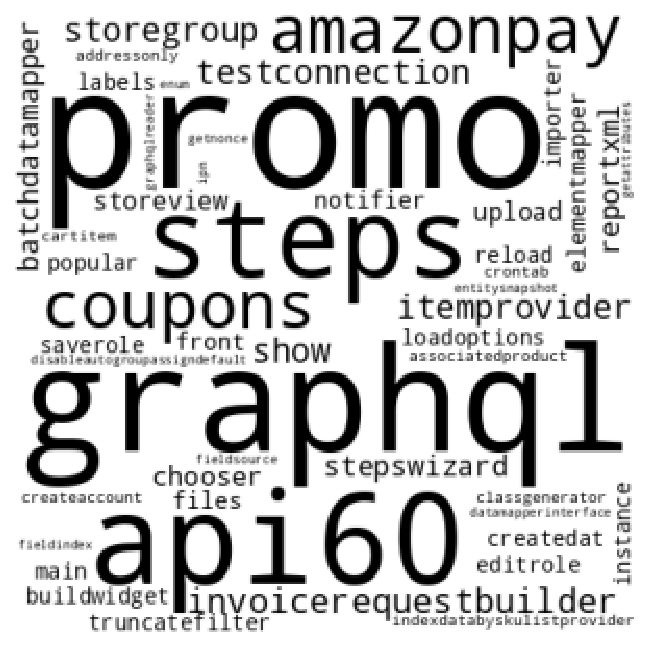
\includegraphics[width=0.5\textwidth]{figures/dbltr/magento_wordcloud.pdf}
%     \caption{Word cloud of important terms for Magento cluster number four}
%     \label{fig:magento_wordcloud}
% \end{figure}

% On the other hand, we observe patterns of feature usage that are unique to a subset of users. 
% Among these user-specific features we observe exporting files with specific file extensions (e.g., CSV), using filters while displaying the query results, and modifying privileges. 
% Similarly, Import/Export, modifying settings such as permalinks, RSS, and WXR are unique to certain clusters among the WordPress users. 
% Finally, for Magento, sales promotions, gifts and shopping cart rules, front end content modification, and sales analytics are among the unique features. 

% We incorporate this observation into our clustering via the max-document-frequency parameter in TF-IDF. 
% This way, we can ignore the common features that are used across all clusters and focus on the unique features when building the clusters. 

% At this step, by looking at the most important terms for each cluster, we can assign a role title to the users of the cluster. 
% Figure~\ref{fig:magento_wordcloud} depicts the word cloud of important terms for a sample cluster of administrators in Magento. 
% Larger font size indicates a higher impact factor based on TF-IDF metric. In general, by analyzing the output of TF-IDF, we can define the following roles for clusters:

% \begin{itemize}
%     \item Mass actions (Delete, Copy, Refresh).
%     \item Invoice, PDF, and Less files.
%     \item Payment methods, Gift cards, and Refunds.
%     \item APIs (GraphQL, XML), Promo, Coupons.
%     \item Index, Cache, Internationalization (i18n).
%     \item Cart, Suggestions, Recommendations.
%     \item Guest purchases, Compare products, Shipping.
% \end{itemize}

\subsection{Debloating results}
%By definition, debloating reduces the effective size of web applications. 
%In this section, we discuss the results of LLOC (Logical Lines of Code), CVE, and CAC (Critical API Call) reduction.

\subsubsection{LLOC Reduction}
 
We measure the reduction in size of web applications in terms of logical lines of code (LLOC), which counts the number of statements in the application source code. 
By reporting the size of the debloated applications in LLOC, we reduce the effects of various syntax and coding styles (i.e., the debloating process changing the code style after rewriting). 

Table~\ref{tab:lloc_reduction} shows the LLOC reduction results of our debloating scheme. 
The numbers are reported in terms of thousands of LLOC. 
The column marked as ``Baseline'' lists the debloating results of combining the code-coverage data of all users together and assigning them to a single role, which is equivalent to prior debloating approaches, such as the one by ``Less is More'' of Amin Azad et al.~\cite{lessismore}.
``\dbltr{}'' shows the LLOC statistics with the optimal number of roles chosen by \dbltr{} for each web application, as discussed in Section~\ref{sec:num-clusters}. 
For \dbltr{} column, we report the size of the role with highest debloated LLOC (Max) and the smallest role with minimum removed LLOC (Min) along with the median. 
The number in the parenthesis for Baseline and \dbltr{} denotes the percentage of LLOC reduction with respect to the size of the original application. 

By comparing the LLOC reduction of Baseline to \dbltr{}, it becomes evident that a one-size-fits-all debloating (i.e., Baseline), exposes certain users and roles to a much larger code-base than they actually require. 
This unnecessary bloat for Baseline debloating can be as high as 30\% of extra LLOC for applications.  
%Nick: This feels like a repetition
%By contrasting the minimum and maximum reduction in \dbltr{} roles, it is evident that in one-size-fits-all debloating schemes certain users would be exposed to a much larger code base than they actually need. 
This unnecessary exposure is most significant for larger web applications such as Magento where certain users inherit up to 90,000 unnecessary LLOC which is 36\% larger---compared to the smallest \dbltr{} role---than what they actually need. 

Moreover, we observe that \emph{all} \dbltr{} roles (including the one with maximum remaining LLOCs) are strictly smaller than the Baseline, meaning that the globally debloated application is still bloated as far as individual users are concerned. 

\begin{table}[t]
    \caption{LLOC reduction of debloated clusters: Numbers are reported in terms of thousands of LLOC. For Baseline, and \dbltr{}, we report the percentage of LLOC reduction compared to the Original application. \dbltr{} columns show the roles with maximum, median and minimum  number of debloated LLOC.}
    \centering
    \adjustbox{max width=\linewidth}{
        \begin{tabular}{|l|l|l|lll|}
            \hline
            \multirow{2}{*}{\textbf{\begin{tabular}[c]{@{}l@{}}Web\\ Application\end{tabular}}} & \multirow{2}{*}{\textbf{Original}} & \multirow{2}{*}{\textbf{Baseline}} & \multicolumn{3}{c|}{\textbf{DBLTR}}                                                  \\ \cline{4-6} 
                                                                                    &                                    &                                    & \multicolumn{1}{l|}{\textbf{Max}} & \multicolumn{1}{l|}{\textbf{Median}} & \textbf{Min} \\ \hline
                phpMyAdmin                                                                          & 155                                & 44 ($\blacktriangledown$72\%)                          & \multicolumn{1}{l|}{32 ($\blacktriangledown$79\%)}    & \multicolumn{1}{l|}{39 ($\blacktriangledown$75\%)}     & 42 ($\blacktriangledown$73\%)     \\ \hline
                WordPress                                                                           & 103                                & 66 ($\blacktriangledown$36\%)                          & \multicolumn{1}{l|}{44 ($\blacktriangledown$57\%)}    & \multicolumn{1}{l|}{54 ($\blacktriangledown$48\%)}    & 64 ($\blacktriangledown$38\%)     \\ \hline
                Magento                                                                             & 1,050                              & 330 ($\blacktriangledown$69\%)                         & \multicolumn{1}{l|}{240 ($\blacktriangledown$77\%)}   & \multicolumn{1}{l|}{270 ($\blacktriangledown$74\%)}   & 326 ($\blacktriangledown$69\%)   \\ \hline
        \end{tabular}
    }
    \label{tab:lloc_reduction}
\end{table}

By comparing the LLOC reduction of Baseline to \dbltr{}, it becomes evident that a one-size-fits-all debloating (i.e., Baseline), exposes certain users and roles to a much larger code-base than they actually require. 
This unnecessary bloat for Baseline debloating can be as high as 30\% of extra LLOC. 
This unnecessary exposure is most significant for larger web applications such as Magento where certain users inherit up to 90,000 unnecessary LLOC which is 37\% larger---compared to the smallest \dbltr{} cluster---than what they actually need. 
Moreover, we observe that \emph{all} \dbltr{} clusters (including the one with maximum LLOCs) are strictly smaller than the Baseline approach, meaning that the globally debloated web application is still bloated as far as individual users are concerned.

\subsubsection{CVE Reduction}

One of the metrics to model the effects of debloating on the security of applications is removal of actual vulnerabilities. 
Historic CVEs provide a good source of information on vulnerabilities and we incorporate a mapping of CVE to source code to identify whether a debloated variant of applications includes the vulnerability or not. 

One of the challenges of this approach is the availability of patch information. 
In order to map a CVE to the vulnerable parts of the source code, we use the data that is available in the form of bug report analysis, Git diffs, and security patches. 
The goal of this step is to identify the files and functions responsible for the vulnerability. 

In our user study, we focused on the latest versions of web applications, so we opted to map all CVEs to these versions. 
In practice, this translates to mapping the location of a CVE to a specific function in a specific file, even if that function is currently patched. 
The purpose of this step is to identify whether the code that contained the vulnerability would have been retained by a debloating approach because it was part of the functionality that the administrators in our user study relied upon.

Some of the web applications in our dataset maintained a stable structure of their source code over time (e.g., WordPress) which makes the process of mapping CVEs from older versions to the recent one straightforward. 
Conversely, phpMyAdmin and Magento changed drastically since their older versions (i.e., Magento version 1.x vs 2.x) and it is not always possible to find the same PHP file/class to perform the mapping. 
Moreover, the developers of phpMyAdmin and WordPress usually acknowledge CVEs in their patches and GitHub commits, whereas for Magento, CVEs are only discussed with minimal details and the patches are released in the form of Major and Minor updates ranging from 500 to 4,000 modifications.

As a result, we mapped 20 CVEs to the source code of phpMyAdmin and WordPress, and mapped 10 recent CVEs to source code of Magento, for a total of 50 mapped CVEs. 
We selected the CVEs with the highest CVSS score, and skipped the ones where the vulnerability or patch information was unavailable. 
The full list of the 50 CVEs that we used in our study along with the information about the \dbltr{} roles such as the number of roles and users that are exposed to each CVE after debloating is available in Table~\ref{tab:cve_details} in the Appendix. 

\begin{figure}[t]
    \centering
    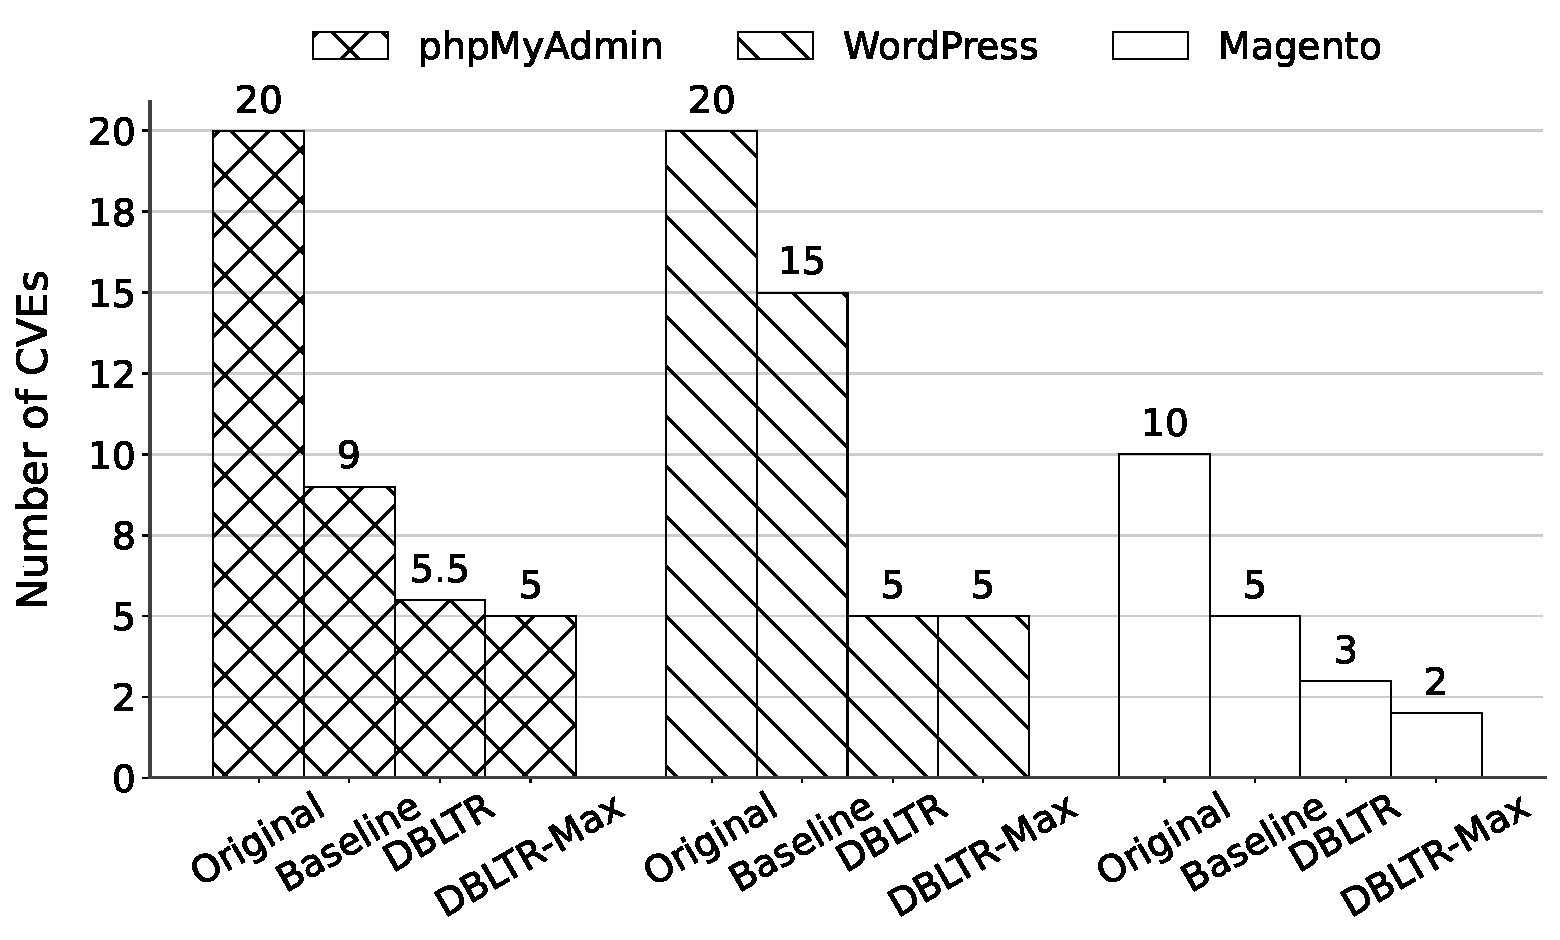
\includegraphics[width=\linewidth]{figures/dbltr/cve_reduction_spectral_bw.pdf}
    \caption{CVE reduction statistics of debloated web applications. ``Original'' represents the total number of mapped CVEs, ``Baseline'' represents the reduction of global debloating, ``DBLTR'' depicts the median reduction across roles, and ``DBLTR-Max'' represents the roles with the highest CVE reduction.}
    \label{fig:cve_reduction}
\end{figure}

Figure~\ref{fig:cve_reduction} depicts the number of CVEs remaining after debloating for each web application. 
The ``\dbltr{}'' bar shows the median CVE reduction across roles, while ``\dbltr{}-Max'' shows the roles with highest CVE reduction representing the maximum protection provided by \dbltr{} for users in those roles. 
For example, for phpMyAdmin we discover that 3/6 roles (accounting for 65\% of users) exposed to the fewest remaining vulnerabilities. 
These roles contained 5 historic CVEs corresponding to 45\% reduction of CVEs compared to the Baseline debloating and 75\% reduction compared to the non-debloated application. 
Similarly, the median number of vulnerabilities among the roles was 5.5 accounting for 40\% reduction compared to the Baseline approach. 
This effect is even more pronounced in WordPress where \dbltr{} reduces the median number of CVEs per role to 4 accounting for a 73\% reduction compared to the 15 CVEs remaining after the Baseline debloating approach. 
Magento exhibits a similar trend of localized debloating gains.

Overall, our results demonstrate that debloating web applications based on clusters of usage-data (i.e., roles) results in significant reduction of severe historic CVEs, compared to prior debloating schemes that could only remove code that was determined to be globally unnecessary for all users of a deployed web application.

\subsubsection{Case Study: phpMyAdmin Database Export Local file Inclusion Vulnerability}

phpMyAdmin version 4.0 is vulnerable to CVE-2013-3240 which resides in the database export functionality. 
This vulnerability allows the attackers to bypass the \texttt{checkParameters} function by sending a specially-crafted variable. 
phpMyAdmin uses this variable to determine the database export file type (e.g., .sql, or .zip) and load the corresponding plugin. 
Malicious users can abuse this flaw to load and execute arbitrary PHP files from the server. 

The export feature in phpMyAdmin is commonly used to backup existing databases and therefore is highly unlikely to be removed by prior global-debloating mechanisms.
Nevertheless, we observed that one of our roles produced by \dbltr{} included four users who did not exercise the export functionality. As a result, \dbltr{} is able to remove this feature from the source code of that specific role, protecting the web application from abuse by these four specific users (including from attackers who compromise their accounts). 

\subsubsection{Critical API Calls Reduction}

Another security metric that we analyze is the reduction in Critical API Calls (CACs). 
Figure~\ref{fig:cac_reduction} depicts the average CAC reduction across all roles. 
The first bar of each group shows the total number of CACs for the Baseline debloating. 
Baseline indicates the reductions in the global debloating scheme where all users are grouped into a single role. 
\dbltr{} bars show the average reduction of CACs based on the optimal number of roles for each web application and \dbltr{}-Max represents the maximum reduction in CACs for a subset of users. 

Across all CAC categories and all web applications, we observe a reduction of 10\% up to 70\% for \dbltr{} debloating. 
This reduction indicates that a sizable number of CACs are in unused parts of the applications. Upon closer inspection of phpMyAdmin results, it becomes evident that 85\% of code execution APIs reside in the external dependencies of the web application, out of which, \dbltr{} removed 12\%-20\%. 
For the larger applications such as Magento, the reduction in Code Execution APIs is more significant where 32\%-53\% of these APIs are removed by \dbltr{}.
Over all categories of CACs, we observe that \dbltr{} removes tens to hundreds of such API calls beyond the Baseline, further protecting web applications from exploits that target these APIs. 

\begin{figure}[t]
    \centering
    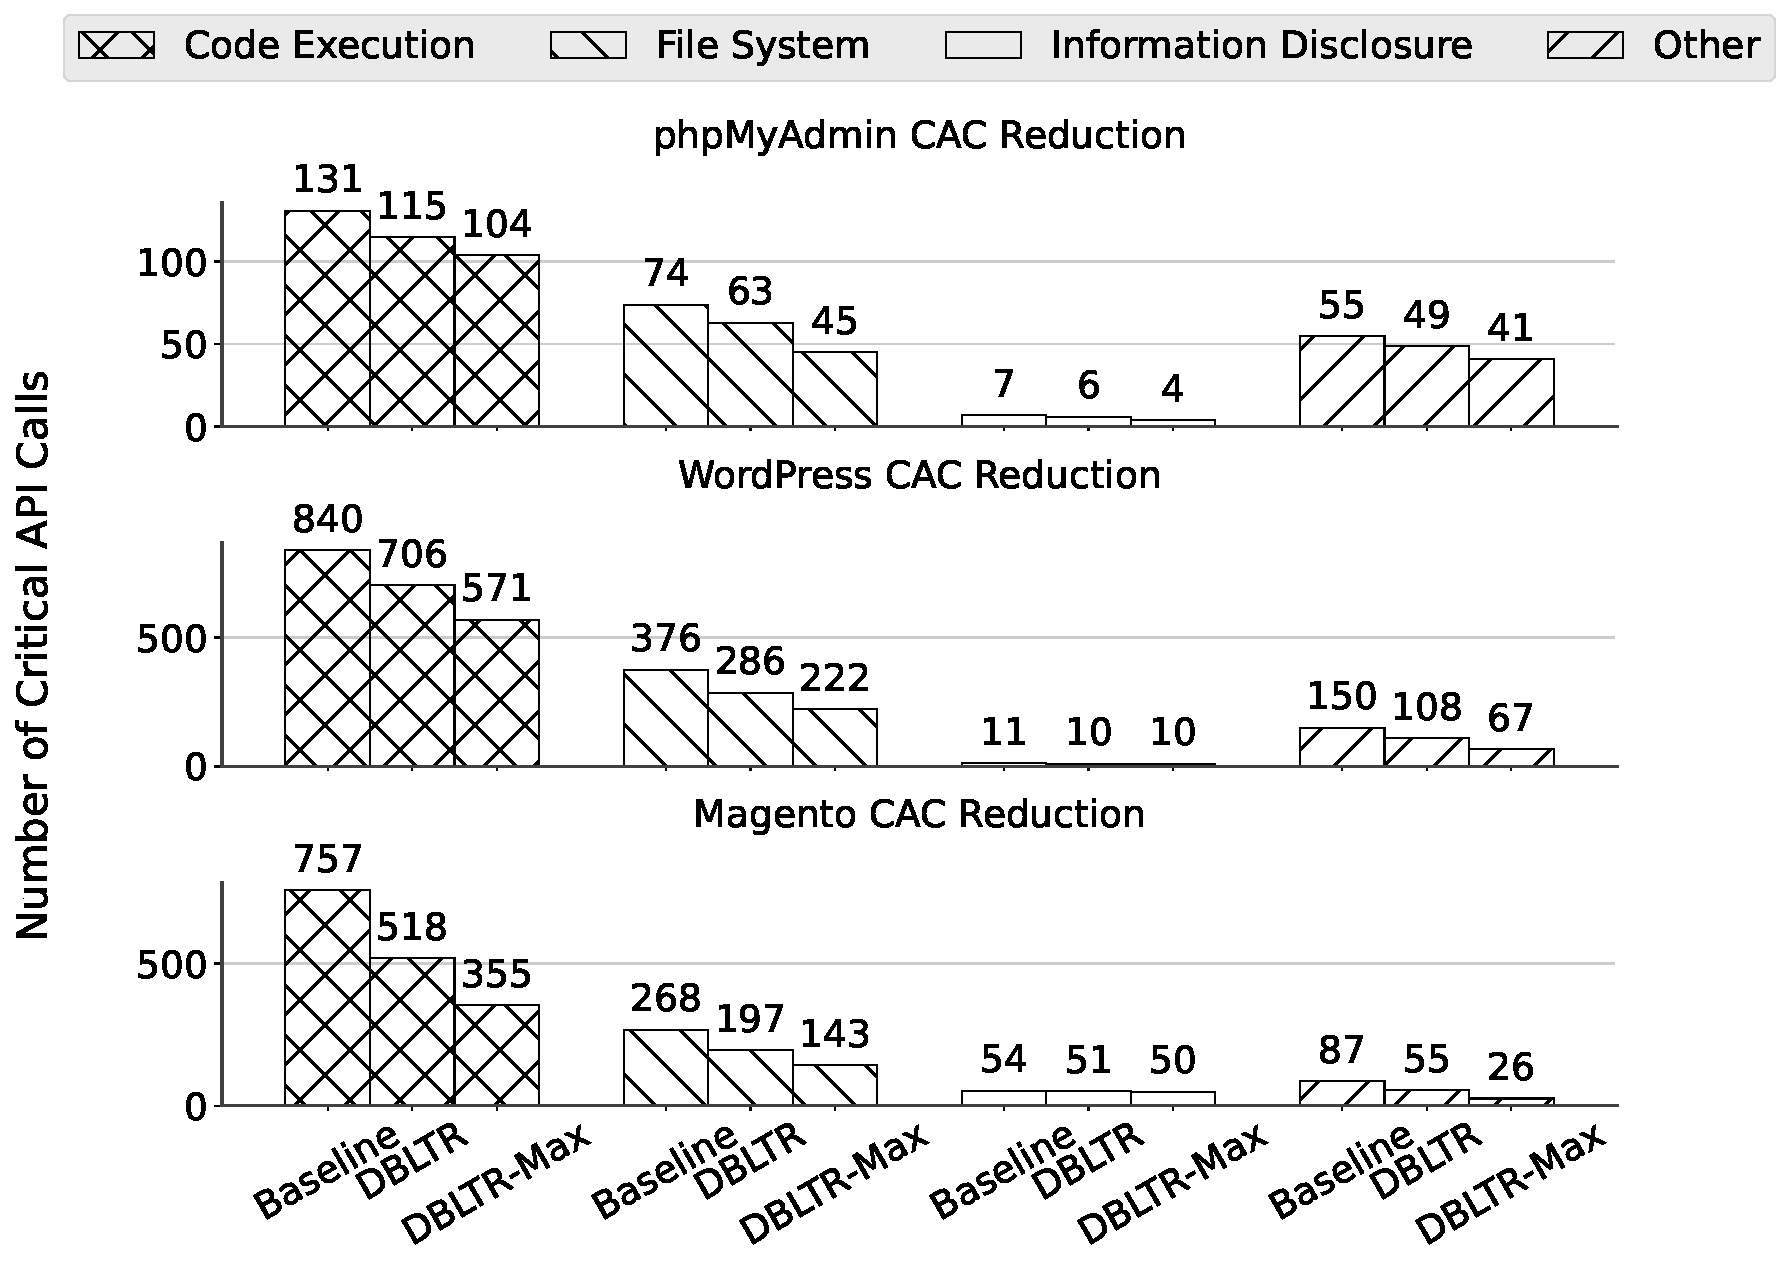
\includegraphics[width=\linewidth]{figures/dbltr/cac_reduction_spectral_bw.pdf}
    \caption{Critical API Call (CAC) reduction after debloating. Baseline represents the global debloating approach where all users are assigned to the same role. \dbltr{} indicates the average reduction across roles.}
    \label{fig:cac_reduction}
\end{figure}

\subsubsection{PHP Object Injection Gadget Reduction}

To identify existing object injection gadgets in the applications, we incorporate PHPGGC~\cite{PHPGGC}, an open-source project listing available gadget chains for popular composer packages. 
After mapping the list of vulnerable package with those in phpMyAdmin, WordPress, and Magento, we search for the removal of classes and functions used within the gadget chains after debloating. 

Table~\ref{tab:poi_gadgets} lists the packages in each of our web applications with a known gadget chain based on PHPGGC. 
Under the column named ``Original'' we list the number of gadget chains within each package. 
As before, the Baseline column lists the number of gadget chains available after the global debloating (i.e., single role), whereas the \dbltr{} column lists the percentage of roles in \dbltr{} exposed to these gadgets. 

The Symfony package in phpMyAdmin includes 2 known gadget chains that can lead to arbitrary file write and code execution. 
Debloating the application into 1-Cluster (Baseline) as well as \dbltr{} debloating remove these gadgets. 
For TCPDF gadget, while the baseline debloating does not remove it, \dbltr{} protects 17\% of the clusters from object injection exploits using this gadget. 
For WordPress, the baseline debloating strategy removes the existing gadget therefore there are no opportunities for any additional gains by \dbltr{}.

More interestingly, Magento contains 10 known gadget chains. 
For Magento's Guzzle package, we observe that while 2 gadgets are still present in the Baseline debloating, one of the gadget chains is fully removed from all roles.
For the gadget chain within the Magento package itself, only (1/7) 14\% of roles produced by the \dbltr{} contain this gadget, therefore, the majority of users are protected.

Our results confirm the findings of previous work that debloating is a highly effective defense for removing publicly known object injection gadget chains. 
Moreover, we observe that by clustering users into multiple groups, we can further breakdown the availability of gadgets and in certain cases, further complicating the exploitation of object injection vulnerabilities. Under a \dbltr{}-protected deployment, attackers not only need to identify the available gadgets in the target web application to build their exploit chain, but they also have to target \emph{specific} victims who have access to the underlying gadgets used in their exploits. 

\begin{table}[t]
    \centering
    \caption{PHP Object Injection Gadgets statistics after debloating. Listing number of existing gadgets for Baseline and the percentage of roles in \dbltr{} exposed to those gadgets.}
    \label{tab:poi_gadgets}
    \scalebox{1}{
        \begin{tabular}{|l|l|c|c|c|}
            \hline
            Web Application             & Package & Original & Baseline & \dbltr{} \\ \hline
            \multirow{2}{*}{phpMyAdmin} & Symfony & 2        & 0        & 0     \\ \cline{2-5} 
                                        & TCPDF   & 1        & 1        & 83\%  \\ \hline
            WordPress                   & Generic & 1        & 0        & 0     \\ \hline
            \multirow{3}{*}{Magento}    & Guzzle  & 3        & 2        & 100\%, 0\% \\ \cline{2-5} 
                                        & Magento & 1        & 1        & 14\%  \\ \cline{2-5} 
                                        & Monolog & 6        & 0        & 0     \\ \hline
            \end{tabular}
    }
\end{table}

% \subsection{Contribution of individual users to the overall code-coverage of clusters}
% \label{sec:augmented_coverage}

% Dynamic code-coverage data precisely models how users interact with web applications. 
% One of the limitations of this modeling is that it overlooks the use cases that it has not seen before. 
% As an example in our dataset, we observed that certain users executed queries that resulted only in a few rows. 
% Therefore, some of the functions within the ``Display Results'' class of phpMyAdmin relating to pagination of results were never invoked. 
% Meanwhile, other users with very similar usage behavior that ended up in the same cluster executed queries that exercised the pagination functions. 
% As a result, all users within this cluster would retain this functionality and can run queries that result in numerous rows.
% In such scenarios, the clustering expands the available features for users with similar usage patterns. 

% To quantify this effect, we look at the contribution of individual users in the cluster compared to the overall cluster code-coverage. 
% For each user, we compare their file and function coverage information with all other users in the same cluster. 
% To identify similar functionality that have been added to the cluster coverage by other users, we look at new lines covered in an already covered file. 
% This modeling captures the effect of exercising new features within an already covered file.
% Moreover, we investigate the inclusion of new files in the overall coverage within an existing module. 
% For this purpose, we closely investigate the source code structure of the web applications in our dataset and identify the directory structure of their internal and external (e.g., composer) packages. 

% \subsubsection{Analyzing module structures} By analyzing the code-base structure of the applications in our dataset, we made the following observations:

% \textbf{phpMyAdmin} uses composer packages. As a result, external dependencies such as Twig, Symfony, Tcpdf, etc. are located under \texttt{vendor/package\_author/package\_name/} directory structure.
% Similarly, phpMyAdmin stores internal modules and classes such as Charsets, Display, Export, etc. under \texttt{libraries/classes/module\_name/}. 
% For phpMyAdmin, we identified 98 external and 23 internal modules.

% \textbf{WordPress} unlike phpMyAdmin, does not use external composer packages. 
% Nevertheless, WordPress modules are split into public and admin sections. 
% Admin modules are located under \texttt{wp-admin/includes/class\_name} and public modules are under \texttt{wp-includes/class\_name}. 
% Some examples of these modules are, PHPMailer, Requests, Rest-API, Widgets, etc.
% Similarly, WordPress themes and plugins have their own unique directory under \texttt{wp-content/themes} and \texttt{wp-content/plugins} directory. 
% For WordPress we identified 23 first-party modules. 

% \textbf{Magento} incorporates multiple first-party and third-party modules via composer. 
% Also, internal modules and classes are located under \texttt{app/code/Magento/module\_name} as well as \texttt{generated/code/module\_name}. 
% From the Magento source code, we identified 493 external and 190 internal modules. 

% Statistics on the code-coverage contribution of clusters to each individual user are available in Table~\ref{tab:augmented_coverage}. 
% Under the column ``\% Files with new coverage'' we report the percentage of total files for which the cluster contributed new lines to the code-coverage of each individual member of that cluster. 
% This number ranges from 15.3\% to 38.3\%, which signifies that a considerable number of functions for each class are included in the final code-coverage by other users in the same cluster. 

% Table~\ref{tab:augmented_coverage} also lists the total number of third-party packages and first-party class modules. 
% Clustering led to inclusion of new files for an average of 29\% to 71\% of packages, and 50\% to 72\% of class modules. 
% On a similar note, these results quantitatively demonstrate that clustering users with similar behavior together leads to inclusion of similar functions, and therefore, reduces the likelihood of removing functions that are actually required by the users. 
% Users who make extensive use of the necessary web-application features cluster together with users with more lightweight usage, allowing the latter to gradually expand their use without breaking the web application due to debloated code. 

% Finally, we look at the number of ``Removed Packages'' for the clusters produced by \dbltr{} in Table~\ref{tab:augmented_coverage}. 
% This column reports the number of packages in the web application where a given percentage of lines are removed after debloating.
% These statistics show that for over half of the packages for phpMyAdmin and Magento, debloating has removed more than 70\% of their lines. 
% In other words, while clustering users with similar behavior together expands their code-coverage of similar features significantly, the debloating procedure is still successfully removing the majority of the code from third-party dependencies, where majority of the bloated code resides~\cite{lessismore}.

\subsection{Performance of \dbltr{}}

We analyze the performance of \dbltr{} from two perspectives, request response time, and server resource utilization. 
Our test setup consists of an HTTP client and the web server. 
The HTTP clients simulate 100 users that send requests in parallel. 
Each client runs in a separate thread and sends batches of 40 requests (average number of requests to load the homepage of WordPress and its resources) towards the main page of WordPress hosted on a remote server. 
This setup simulates the work load for a website with 192,000 daily page views receiving 90 requests-per-second. 
We run each test for five minutes and repeat the tests five times and report the average statistics and remove the outliers. 

For the server setup, our web server hosts a WordPress website and we run each configuration in a containerized environment. 
We run our web servers on a server with 32GBs of RAM, and 32 Cores of Intel Xeon E5-2440 v2 CPUs running Ubuntu 18.04 LTS. 
We test the following setups:

\begin{itemize}
    \item \textbf{Single web server (Apache)} consists of one Apache web server without a reverse-proxy. 
    \item \textbf{Baseline} is made up of an OpenResty reverse proxy and one Apache web server. This setup serves as our baseline. 
    \item \textbf{\dbltr{} setups} expand the baseline setup by including the \dbltr{} modules and consist of one reverse-proxy and 1-50 Apache web servers. Each web server is responsible for the debloated web application for a specific role. This way, we measure the effect of the number of roles on the request response times. Under this setup, each client is assigned to one role in a round-robin fashion.
\end{itemize}

\begin{figure}[]
    \centering
    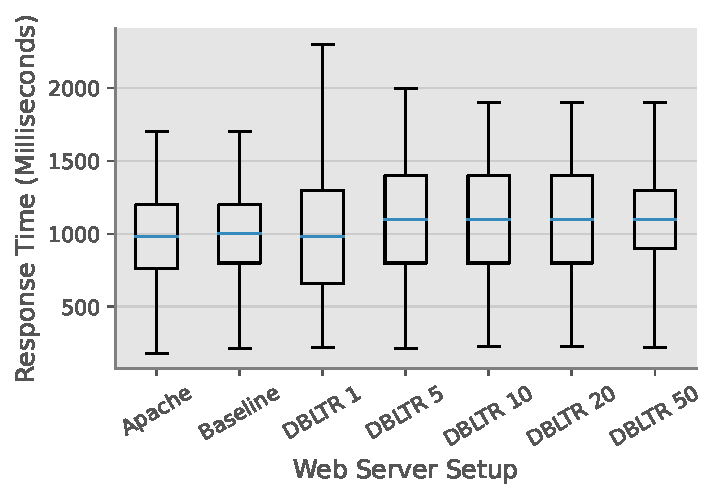
\includegraphics[width=0.8\linewidth]{figures/dbltr/performance.pdf}
    \caption{Distribution of request response time in milliseconds for Apache, Baseline, and \dbltr{} with a varying number of roles (i.e., backed Apache servers).}
    \label{fig:performance}
  \end{figure}

\subsubsection{Request Response Time Statistics}
We measure the request response time statistics from the perspective of our HTTP clients and report them in Figure~\ref{fig:performance}. 
The mere addition of the reverse-proxy (Baseline) increases the median response time of requests by 2\%. 
For \dbltr{}, the overhead from analysis and routing modules results in an average increase of 12\% in the median response time and 15\% increase in the 99th percentile response time. 
Moreover, a higher number of roles reduces the variance in the response times, as evident by the smaller boxes and shorter whiskers from one (DBLTR 1) to fifty roles (DBLTR 50). 

\subsubsection{Resource Utilization}
We measured the CPU and memory utilization of our test setup using the Docker runtime metrics API. 
Table~\ref{tab:performance} reports the resource usage statistics for the web servers and content-delivery (i.e., reverse-proxy) modules. 
Overall, the content-delivery module both in baseline and \dbltr{} setups utilizes 5-6\% of CPU and less than 20~MiB of RAM which is very small compared to the amount of resources utilized by the web server. 
Moreover, across all setups, the CPU utilization of the web server modules remains constant. 
At the same time, increasing the number of roles in \dbltr{} which results in an increase in the number of web servers results in a linear increase in the overall memory utilization. 
During our tests, we observed a 5x increase in overall memory usage of \dbltr{}'s web servers when increasing the number of roles by an order of 50x. 

\paragraph{Disk space utilization} \dbltr{} stores a separate and unique debloated copy of the web applications for each role. 
As a result, the disk utilization overhead of \dbltr{} is proportional to the number of roles. 
While shrinking the disk utilization of \dbltr{} is not a main goal, by definition, the debloating process removes unused lines of code. 
Overall, debloated web applications occupy 5-10\% less disk space. 
While this reduction may be insignificant for smaller web applications, for larger ones such as Magento, debloated web applications on average occupy 100~MB less disk space. 


\begin{table}[]
    \centering
    \caption{Average CPU and Memory utilization of \dbltr{}. \textit{DBLTR N}-Web Servers row shows the range of CPU and Memory utilization for \textit{DBLTR 1} to \textit{DBLTR 50}.}
    \label{tab:performance}
    \adjustbox{max width=\columnwidth}{
    \begin{tabular}{|l|l|l|l|}
    \hline
    \textbf{Setup}                    & \textbf{Module}  & \textbf{Avg CPU} & \textbf{Avg Memory (MiB)} \\ \hline
    Apache                            & Web Server       & 3,117\%              & 2,378                            \\ \hline
    \multirow{2}{*}{Baseline}         & Content-Delivery & 6\%                 & 17                           \\ \cline{2-4} 
                                      & Web Server       & 3057\%              & 2,332                         \\ \hline
    \multirow{2}{*}{\textit{DBLTR N}} & Content-Delivery & 6\%                 & 19                           \\ \cline{2-4} 
                                      & Web Servers      & 2,905-3,072\%      & 2,179-10,374                \\ \hline
    \end{tabular}
    }
\end{table}